\documentclass[12pt]{article}
\usepackage{verbatim}
\usepackage[dvips]{epsfig}
\usepackage{color}
\usepackage{url}
\usepackage[colorlinks=true]{hyperref}

\begin{document}

\section*{GENESIS: Documentation}

{\bf Related Documentation:}
% start: userdocs-tag-replace-items related-do-nothing
% end: userdocs-tag-replace-items related-do-nothing

\section*{g-tube Development Design}

	This document outlines the design process employed in the development of the {\bf g-tube}, a graphical user interface which brings all components of the {\bf GENESIS3} system together. With the {\bf g-tube} a user can load, create and run models, track all aspects of the simulation including the schedule, parameters, models, underlying software versions, and directly load the output of simulation runs into {\bf Atoms} that can be processed into tables, plots, and formatted text suitable for inserting into publications. The end result of a {\bf g-tube project} will be a compiled electronic publication, containing the finalized document, with all of the data used to generate the figures {\bf tag-associated}  with the model experiment runs.


\section*{Data Design}

\subsection*{Project Specification}

	A project is a class data structure that is used to track all work done by the user within the {\bf g-tube}. Projects are treated as a combination of categorized lists of data that grow and shrink as the user works. Data tracked includes:
	
\begin{itemize}
	\item[] Project name.
	\item[] List of associated models.
	\item[] List of working atoms.
	\item[] List of publication atoms.
	\item[] Publication pages.
	\item[] GUI perspective state.
\end{itemize}

From a file storage perspective a project consists of a directory containing all files in the users workspace along with a {\bf yaml} file that bears the same name as the project. The {\bf yaml} file provides a mapping for all of the files in the project directory so that they can be loaded by the appropriate data management objects within the GUI.

\subsection*{Object Relationships}

	The {\bf g-tube} is set up with a set of "management" classes; their purpose is to provide high level control for the GUI to work with all of the underlying systems, without allowing code from unrelated systems to interlace with one another.

\begin{itemize}
	\item[] {\bf Project Manager:} Loads or creates a project specification and allows for creating, deleting and editing Model, Atom, Publication, and Review management objects.
	\item[] {\bf Model Manager:} Manages a list of models associated with the current project.
	\item[] {\bf Atom Manager:} Manages a list of all of the working atoms in the current project. 
	\item[] {\bf Publication Manager:} Manages the atoms tagged as part of a publication.
	\item[] {\bf Review Manager:} Manages the compiled publication atoms for review.
\end{itemize}

The management objects allows for basic list operations such as adding, deleting, and editing members. Management objects encapsulate {\bf wxPython} operations for allowing the end user to perform these actions graphically.


\section*{Architecture Design}

Working.


\section*{Interface Design}

\subsection*{UI Real Estate}

Presentation of widgets is implemented with the {\bf wxPython} Advanced User Interface (AUI) toolkit. This allows for several dockable panes that the user can rearrange to their liking. 

\begin{figure}[ht]
   \centering
   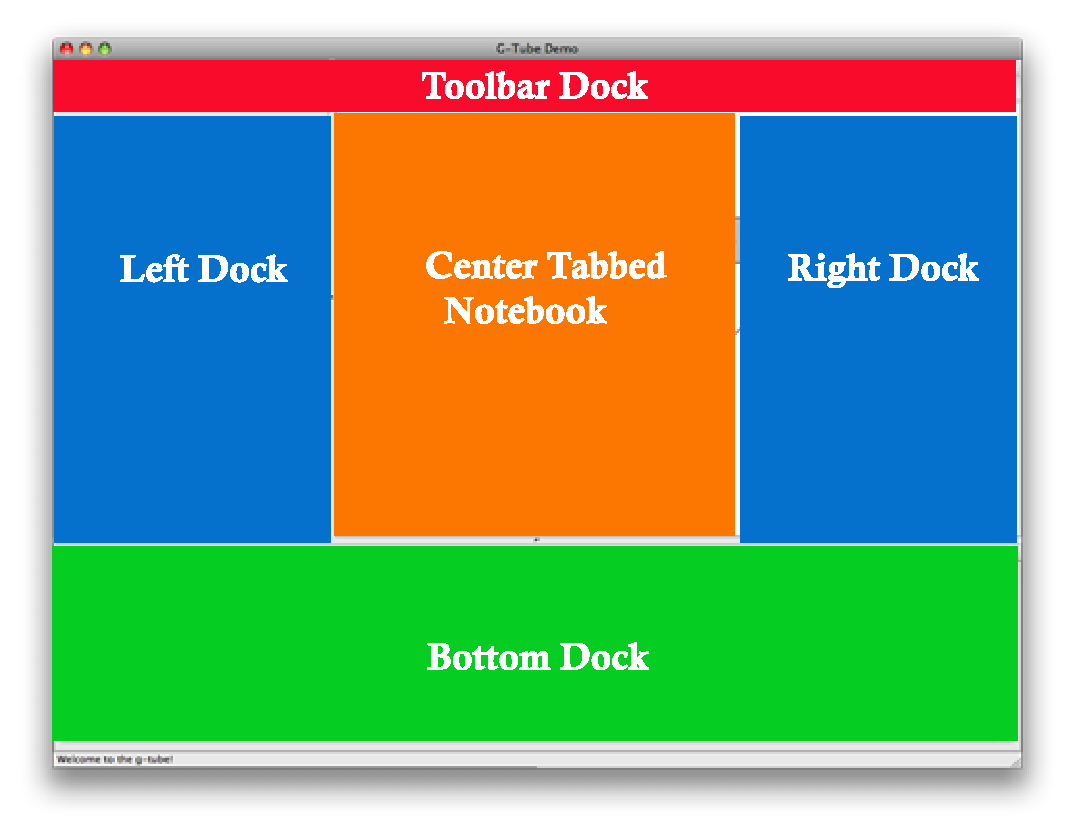
\includegraphics[scale=0.6]{figures/RealEstate.eps}
   \caption{{\bf Main Frame Layout:} Figure shows the default layout of the frames dockable panels.}
   \label{fig:Real Estate}
\end{figure}

\begin{itemize}
\item[] {\bf Toolbar Dock:} Holds icon labeled buttons for performing many shortcuts within the system. Toolbars can be removed from the dock and allows to float at different areas of the screen.
\item[] {\bf Left Dock:} The primary dock for explorer widgets used to manage data in the {\bf Model}, {\bf Atom}, {\bf Publication}, and {\bf Review} workspaces.
\item[] {\bf Center Tabbed Notebook:} The "main" workspace. All data selected from a workspace via an explorer will be displayed in a Tab in the Center Notebook. E.G Editable Documents, Publication Atoms, Plots from simulation.
\item[] {\bf Right Dock:} Primarily used to hold widgets for editing attributes (such as tags) to the current working tab in the Center Notebook.
\item[] {\bf Bottom Dock:} Primarily holds widgets that output data from the underlying system. E.G Console output from the {\bf g-tube}, model status, error messages.
\end{itemize}




\section*{Procedural Design}

Working.








\begin{itemize}
\item[]  {\bf The Documentation Identifier:} This may be replaced by a descriptor of the type of documentation you have developed, for example {\bf Introduction} or {\bf Tutorial}, etc.
\item[]{\bf Related Documentation Heading:} Followed by a hyperlink list of any related documentation.
\item[] {\bf New Document Heading:} Should be replaced with the title of your document. {\bf Note:} In your document (the \LaTeX\,\,source documentation file--{\it NewDocument.tex}) all text below the {\bf New Document} heading should be replaced with your own content. See \href{../document-create/document-create.tex}{\bf Create\,Document} for further information.
\end{itemize}

\subsection*{Help with \LaTeX\,Documentation}

\subsubsection*{Text color}

Text in your document can be colorized  with the command
\begin{verbatim}
    \textcolor{red}{text}
\end{verbatim}
for example \textcolor{red}{\bf This is IMPORTANT}, \textcolor{green}{green} and \textcolor{blue}{blue} are also recognized arguments.

\subsubsection*{Hyperlinks}

Two classes of hyperlink exist in the GENESIS Documentation System:

\begin{itemize}
\item[{\bf A.}]{\bf Static Hyperlinks:} 
   \begin{itemize}
      \item{\bf Local links:} These are produced with the command:
\begin{verbatim}
   \href{../NewDocument/NewDocument.tex}{NewDocument}}
\end{verbatim}
for example \href{../NewDocument/NewDocument.tex}{NewDocument} references this document.
Note that these links may not work in your \LaTeX\,{\tt pdf} file viewer, but should be testable with the \href{http://get.adobe.com/reader/}{Acrobat Reader} or \href{http://www.adobe.com/products/acrobatpro/tryout.html}{Acrobat Professional} packages.
      \item {\bf Remote links:} These use the {\tt href} command in a slightly different way:
\begin{verbatim}
    \href{http://www.genesis-sim.org/documentation}{GENESIS Documentation}
\end{verbatim}
for example see \href{http://www.genesis-sim.org/documentation}{GENESIS Documentation}. Note that these links do not wrap automatically at the end of a line even outside of the {\tt verbatim} environment.
\end{itemize}

\item[{\bf B.}]{\bf Reference Hyperlinks:} See \href{../document-create/document-create.tex}{Document Creation} for further details on managing reference hyperlinks.

\end{itemize}

\subsubsection*{Figures}

Figures can easily be added with the following code:

\begin{verbatim}
\begin{figure}[h]
   \centering
   
\includegraphics[scale=0.6]{figures/dummyfig.eps}
   \caption{{\bf A Dummy Figure:} Example of Latex code to incorporate
      a figure into documentation.}
   \label{fig:df-1}
\end{figure}
\end{verbatim}

\bibliographystyle{plain}
\bibliography{../tex/bib/g3-refs.bib}

\end{document}
